\documentclass[11pt,a4paper]{article}
\usepackage[utf8]{inputenc}
\usepackage[T1]{fontenc}
\usepackage{amsthm} %numéroter les questions
\usepackage[english]{babel}
\usepackage{datetime}
\usepackage{xspace} % typographie IN
\usepackage{hyperref}% hyperliens
\usepackage[all]{hypcap} %lien pointe en haut des figures
\usepackage[french]{varioref} %voir x p y
\usepackage{fancyhdr}% en têtes
%\input cyracc.def
\usepackage[]{graphicx} %include pictures
\usepackage{pgfplots}
\usepackage[]{circuitikz}
\usepackage{ifthen}

\usepackage[top=1.3 in, bottom=1.3 in, left=1.3 in, right=1.3 in]{geometry} % Yeah, that's bad to play with margins
\usepackage[]{pdfpages}

\usepackage[]{attachfile}

\usepackage{float}
\usepackage{subfig}

\usepackage{todonotes} % \missingfigure
\usepackage{gensymb} % \ohm

\usepackage{framed}

\newdateformat{mydate}{v1.0.0}%hack pour remplacer \THEYEAR


\newboolean{corrige}
\ifx\correction\undefined
\setboolean{corrige}{false}% pas de corrigé
\else
\setboolean{corrige}{true}%corrigé
\fi

%\setboolean{corrige}{false}% pas de corrigé

\newboolean{annexes}
\setboolean{annexes}{true}%annexes
%\setboolean{annexes}{false}% pas de annexes

\definecolor{darkblue}{rgb}{0,0,0.5}

\newboolean{mos}
%\setboolean{mos}{true}%annexes
\setboolean{mos}{false}% pas de annexes

\usepackage{aeguill} %guillemets

%% fancy header & foot
\pagestyle{fancy}
%Numero du TP :
\def \labonumber {Projet -- Part 3}
\lhead{[ELEC-H-310] Choucroute numérique\\ \labonumber}
\rhead{\mydate\today\\ page \thepage}
\chead{\ifthenelse{\boolean{corrige}}{Corrigé}{}}
\cfoot{}
%%

\pdfinfo{
/Author (Quentin Delhaye, Ken Hasselmann, ULB -- BEAMS)
/Title (\labonumber ELEC-H-310)
/ModDate (D:\pdfdate)
}

\hypersetup{
pdftitle={\labonumber [ELEC-H-310] Choucroute numérique},
pdfauthor={Quentin Delhaye, Ken Hasselmann, ULB -- BEAMS},
pdfsubject={}
}

\theoremstyle{definition}% questions pas en italique
\newtheorem{Q}{Question}[] % numéroter les questions [section] ou non []

\newcommand{\reponse}[1]{% pour intégrer une réponse : \reponse{texte} : sera inclus si \boolean{corrige}
	\ifthenelse {\boolean{corrige}} {\paragraph{Réponse :} \color{darkblue}   #1\color{black}} {}
 }

\newcommand{\addcontentslinenono}[4]{\addtocontents{#1}{\protect\contentsline{#2}{#3}{#4}{}}}

\date{\vspace{-1.7cm}\mydate\today}
\title{\vspace{-2cm}\labonumber\\ Électronique numérique [ELEC-H-310]\\Conception d'une régulation de refroidissement: \\ interactions avec l'utilisateur\ifthenelse{\boolean{corrige}}{~\\Corrigé}{}}

\title{\vspace{-2cm}\labonumber \\ Digital electronics [ELEC-H-310]\\Design of a cooling control system: \\ interactions with user\ifthenelse{\boolean{corrige}}{~\\Corrigé}{}}

%\author{\vspace{-1cm}}%\textsc{Yannick Allard}}

\setlength{\parskip}{0.2cm plus2mm minus1mm} %espacement entre §
\setlength{\parindent}{0pt}


















\begin{document}
\pagestyle{empty}
\maketitle
% \vspace*{-1cm}




% ########   ##     ##  ##########  
% ##     ##  ##     ##      ##      
% ##     ##  ##     ##      ##      
% ########   ##     ##      ##      
% ##     ##  ##     ##      ##      
% ##     ##  ##     ##      ##      
% ########    #######       ##      

\section*{But de la manipulation}
During three laboratory sessions, you will have to design a small cooling control system based on a propeller fan.
You will also have to be able to interact locally (keyboard) with this system.

During this third lab session, you will add two interaction modes between the temperature control system and the user: either locally with a keyboard, or remotely through a serial port.

At the end of this lab session, you should finish your whole cooling control system.


\section*{Prerequisite}
Before entering in the lab, you have to read the project specifications defined in the document ``Design of a temperature regulation system".



\section*{Objectifs}
At the end of this lab session, you'll be able to:
\begin{itemize}
	\item Design and implement a serial connection between two processors and to explain how it works.
	\item To make numerous peripheral devices communicate with each other.
\end{itemize}


\newpage





% ########   ##      ##  ##########  ########     #####    
%    ##      ###     ##      ##      ##     ##  ##     ##  
%    ##      ## ##   ##      ##      ##     ##  ##     ##  
%    ##      ##  ##  ##      ##      ########   ##     ##  
%    ##      ##   ## ##      ##      ##   ##    ##     ##  
%    ##      ##     ###      ##      ##    ##   ##     ##  
% ########   ##      ##      ##      ##     ##    #####    


\section{Introduction}
During three laboratory sessions, you will have to design a small cooling control system based on a propeller fan.
You will also have to be able to interact locally (keyboard) with this system.

During this lab session, you will first build a way to interact with the keyboard of the extension PCB.
Depending on the character string in input, different changes will have to be forecast in the operating of the PCB (ex: change of the desired temperature, of the sampling period, ...).

Then, you will ensure than similar changes could be done... remotely!
A PC, connected to the processor through a serial cable, will play the role of the control room allowing you to interact with the processes without being physically present.






%  #######   ##            ###     ##     ##  ########   #########  ########   
% ##     ##  ##           ## ##    ##     ##     ##      ##         ##     ##  
% ##         ##          ##   ##   ##     ##     ##      ##         ##     ##  
% ##         ##         ##     ##  ##     ##     ##      ######     ########   
% ##         ##         #########   ##   ##      ##      ##         ##   ##    
% ##     ##  ##         ##     ##    ## ##       ##      ##         ##    ##   
%  #######   #########  ##     ##     ###     ########   #########  ##     ##  



\section{Keyboard interfacing}
\begin{figure}[H]
\center
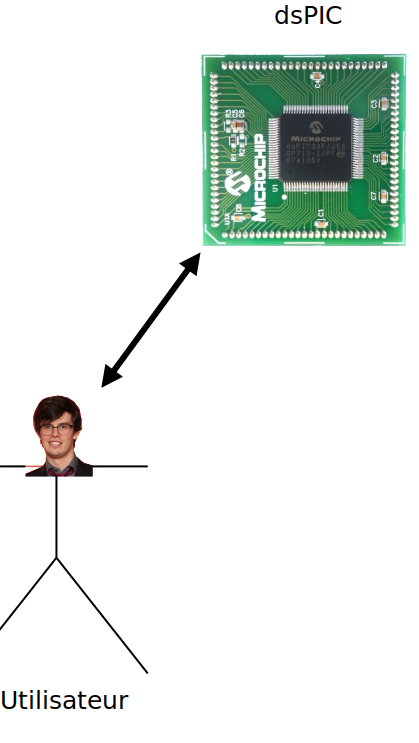
\includegraphics[width=0.3\textwidth]{utilisateur}
\caption{Interaction netween the user and the system.}
\label{fig:user}
\end{figure}

As explained in the coding guide, the keyboard is connected to generic I/O pins of the $\mu$C.
A function allowing to receive the pressed key will be provided.


\begin{itemize}
	\item Thanks to the coding guide, explain the general principal of this ``matrix" keyboard.
	\item During the initializing phase of your code, set correctly the I/O pins connected to the keyboard.
	\item A function allowing you to read the pressed key is given.
	If the key is effectively pressed, it sents the corresponding character (‘0’ to ‘9’ or ‘A’ to ‘F’).
	Otherwise, it sents the value ‘z’.
	\item Look over the code of this function, and explain how it works.
\end{itemize}

Now that the keyboard is working, you can write the function allowing to modify the behaviour of your temperature control center depending on which keys are pressed.
The list of the possible commands is given in the global project specifications.
\begin{itemize}
	\item The function allowing you to read the pressed keys requires a large amount of instructions.
	Where do you have to call this function in order to avoid blocking the processor uselessly?
	\item When the user is typing on the keyboard, the LCD has to display the pressed key.
	Once the command is entered or cancelled, the LCD has to display the temperature again.
\end{itemize}







%  #######   #########  ########   ########   #########  
% ##     ##  ##         ##     ##     ##      ##         
% ##         ##         ##     ##     ##      ##         
%  #######   ######     ########      ##      ######     
%        ##  ##         ##   ##       ##      ##         
% ##     ##  ##         ##    ##      ##      ##         
%  #######   #########  ##     ##  ########   #########  


\section{Serial connection}
In this part, you will send data to the PC through the serial port in order to follow the temperature evolution, as well as to receive the commands from the PC to adjust the temperature control.

The last module to set is the serial port, allowing to communicate remotely with a PC.
This module is named UART (Universal Asynchronous Receiver / Transmitter).

Before designing this communication, you will have to set the dsPIC and the PC in order to make them ``speak the same language".
We will start by the dsPIC setup.

\begin{itemize}
	\item Thanks to the coding guide, configure the UART such that the communication respects the following format:
	\begin{itemize}
		\item Baudrate: 9600
		\item Data bits: 8
		\item No parity bit
		\item Only one stop bit
		\item No stream control
	\end{itemize}
	\item Give the meaning of those parameters.
\end{itemize}

\subsection{Sending data to the PC}
To send the data, 
Pour envoyer des données, refer to the code \texttt{initUART} given as an example and to the coding guide.
As mentioned in the project specifications, you have to sent five characters for each temperature measure: ``42.5\textbackslash n", where ``\textbackslash n" is the character for line break.

To display the data on the PC, you just have the execute the script \texttt{graph.py}.



\subsection{Sending commands from the PC}

On the PC, open the program \texttt{putty}, and set the same format parameters.


Finally, all that remains is to set up the $\mu$C so that it can accept commands coming from the serial port.
\begin{itemize}
	\item Write a routine allowing to read the last character received.
	Justify why this routine must be called with an interruption.
	\item Check if you $\mu$C is capable of receiving a character coming from the PC.
	\item Complete your routine in order to make your system behave as described in the global project specifications.
\end{itemize}






%  #######   ##     ##   #######   ##########    #####    ##       ##  
% ##     ##  ##     ##  ##     ##      ##      ##     ##  ###     ###  
% ##         ##     ##  ##             ##      ##     ##  ## ## ## ##  
% ##         ##     ##   #######       ##      ##     ##  ##  ###  ##  
% ##         ##     ##         ##      ##      ##     ##  ##       ##  
% ##     ##  ##     ##  ##     ##      ##      ##     ##  ##       ##  
%  #######    #######    #######       ##        #####    ##       ##  



\section{Project customization}
Your cooling control system is now functional, you can add different features to enhance it!


\end{document}
